\notechapter{N-20210621}{Prop Presentations for Linear Algebra: Diagrams, Matrices, and Relations}

\newcommand{\wireone}{%
\begin{tikzpicture}[baseline=-0.55ex,scale=0.5]
  \draw (0,0) -- (0,1.4);
\end{tikzpicture}%
}
\newcommand{\copygen}{%
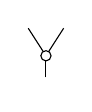
\begin{tikzpicture}[baseline=-0.55ex,scale=0.5]
  \draw (0,0) -- (0,0.55);
  \draw (0,0.55) -- (-0.45,1.25);
  \draw (0,0.55) -- (0.45,1.25);
  \draw[fill=white] (0,0.55) circle (0.13);
\end{tikzpicture}%
}
\newcommand{\discardgen}{%
\begin{tikzpicture}[baseline=-0.55ex,scale=0.5]
  \draw (0,0) -- (0,0.95);
  \draw[fill=white] (0,1.05) circle (0.15);
\end{tikzpicture}%
}
\newcommand{\addgen}{%
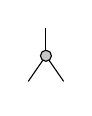
\begin{tikzpicture}[baseline=-0.55ex,scale=0.5]
  \draw (-0.45,0) -- (0,0.65);
  \draw (0.45,0) -- (0,0.65);
  \draw (0,0.65) -- (0,1.35);
  \draw[fill=gray!45] (0,0.65) circle (0.14);
\end{tikzpicture}%
}
\newcommand{\zerogen}{%
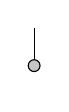
\begin{tikzpicture}[baseline=-0.55ex,scale=0.5]
  \draw (0,0.35) -- (0,1.25);
  \draw[fill=gray!45] (0,0.3) circle (0.15);
\end{tikzpicture}%
}
\newcommand{\scalargen}[1]{%
\begin{tikzpicture}[baseline=-0.55ex,scale=0.5]
  \draw (0,0) -- (0,0.45);
  \node[draw,minimum width=0.45cm,minimum height=0.33cm,inner sep=0pt,fill=white] at (0,0.72) {\scriptsize #1};
  \draw (0,0.9) -- (0,1.35);
\end{tikzpicture}%
}

\section{First orientation}

A deceptively small diagram---a few white nodes, a few grey nodes, scalar labels, and wires---can present linear algebra as a graphical calculus rather than merely serve as a mnemonic.

The central contrast is:
\[
\begin{array}{c}
  \text{ordinary linear algebra writes maps as grids of numbers;}\\
  \text{graphical linear algebra writes them as processes made of wires and nodes.}
\end{array}
\]
This note decodes that special symbolic system.  The point is not to admire the pictures, but to understand why the pictures form a proof system.

The guiding slogan is:
\[
  \text{matrices are compiled diagrams, and diagrams are structured linear processes.}
\]
Once this is understood, the later movement toward linear relations, Lagrangian relations, circuits, and stabilizer calculi becomes much less mysterious.

\section{Props as typed wiring diagrams}

The right ambient language is a prop.

\begin{definition}[Prop]
A prop is a strict symmetric monoidal category whose objects are natural numbers
\[
  0,1,2,\ldots
\]
and whose monoidal product on objects is addition.
\end{definition}

The object \(n\) should be read as \(n\) parallel wires.  A morphism
\[
  f:n\to m
\]
is a process with \(n\) input wires and \(m\) output wires.

There are two basic operations on morphisms.

First, vertical composition plugs outputs into inputs:
\[
  f:n\to m,\qquad g:m\to p,\qquad g\circ f:n\to p.
\]
Second, the monoidal product puts diagrams side by side:
\[
  f:n\to m,\qquad g:n'\to m',\qquad f\oplus g:n+n'\to m+m'.
\]

This makes a prop feel like a typed programming language for wiring diagrams:
\[
\begin{array}{c|c}
\text{prop notation} & \text{programming / wiring intuition}\\
\hline
n & n\text{ wires}\\
f:n\to m & \text{process with }n\text{ inputs and }m\text{ outputs}\\
g\circ f & \text{run }f\text{, then run }g\\
f\oplus g & \text{run }f\text{ and }g\text{ in parallel}
\end{array}
\]

The prop \(\mathbf{Mat}_k\) has natural numbers as objects and matrices over \(k\) as morphisms.  A morphism
\[
  n\to m
\]
is an \(m\times n\) matrix, regarded as a linear map
\[
  k^n\to k^m.
\]
Composition is matrix multiplication, and the monoidal product is block direct sum.

\section{The alphabet: copy, discard, add, zero, and scalars}

The graphical calculus \(\mathbf{cb}_k\) is generated by a small alphabet.  In the diagrams below, time flows upward: inputs are at the bottom and outputs are at the top.

\begin{center}
\small
\begin{tabular}{>{\raggedright\arraybackslash}p{0.16\textwidth}>{\raggedright\arraybackslash}p{0.12\textwidth}>{\raggedright\arraybackslash}p{0.22\textwidth}>{\raggedright\arraybackslash}p{0.34\textwidth}}
\toprule
symbol & type & linear meaning & intuition\\
\midrule
\copygen\quad copy \(\Delta\) & \(1\to2\) & \(x\mapsto(x,x)\) & duplicate one wire into two copies\\
\discardgen\quad discard \(\epsilon\) & \(1\to0\) & \(x\mapsto *\) & forget the value on a wire\\
\addgen\quad add \(\mu\) & \(2\to1\) & \((x,y)\mapsto x+y\) & combine two wires by addition\\
\zerogen\quad zero \(\eta\) & \(0\to1\) & \(*\mapsto0\) & create the additive zero\\
\scalargen{a}\quad scalar \(a\) & \(1\to1\) & \(x\mapsto ax\) & multiply a wire by \(a\in k\)\\
\bottomrule
\end{tabular}
\end{center}

One must be careful about the word ``copy.''  In ordinary vector spaces, there is no natural linear map \(V\to V\oplus V\) for every abstract vector space \(V\) unless one has fixed the diagonal map.  In this prop, one wire represents the free rank-one module \(k\).  The copy generator is the linear map
\[
  k\to k\oplus k,\qquad x\mapsto(x,x).
\]
Arbitrary matrices are then built by composing and tensoring these elementary maps.

\section{Two colours: a comonoid and a monoid}

The white structure is the copying structure:
\[
  \Delta:1\to2,\qquad \epsilon:1\to0.
\]
Algebraically, it is a commutative comonoid.  The equations say that copying twice does not depend on which copy is copied first, that the two copies can be swapped, and that discarding a copied output returns the original wire.

The grey structure is the adding structure:
\[
  \mu:2\to1,\qquad \eta:0\to1.
\]
Algebraically, it is a commutative monoid.  The equations say that adding three terms does not depend on bracketing, that order does not matter, and that adding zero changes nothing.

A good way to remember the two colours is:
\[
\begin{array}{c|c|c}
\text{colour} & \text{structure} & \text{operation}\\
\hline
\text{white} & \text{comonoid} & \text{copy / discard}\\
\text{grey} & \text{monoid} & \text{add / zero}
\end{array}
\]
The calculus becomes interesting because these two structures are not independent.  They interact through the bialgebra law.

\section{The bialgebra law}

The central equation says:
\[
  \text{copy after add}=	ext{add after copying both inputs.}
\]
In ordinary algebra, this is the statement
\[
  \Delta(x+y)=(x+y,x+y)=(x,x)+(y,y).
\]

The two sides can be read as dataflow programs.

Left side:
\begin{verbatim}
input:  (x, y)
step 1: add       -> x + y
step 2: copy      -> (x + y, x + y)
output: (x + y, x + y)
\end{verbatim}

Right side:
\begin{verbatim}
input:  (x, y)
step 1: copy x and copy y       -> (x, x, y, y)
step 2: swap the middle wires   -> (x, y, x, y)
step 3: add pairwise            -> (x + y, x + y)
output: (x + y, x + y)
\end{verbatim}

This is the first moment where the topology of wires matters.  The swap of the middle wires is not decoration.  It is the wiring needed to pair the first copy of \(x\) with the first copy of \(y\), and the second copy of \(x\) with the second copy of \(y\).

\begin{remark}
The bialgebra law is the graphical form of distributivity.  It says that copying respects addition.  Without this law, the white and grey nodes would be two unrelated gadgets; with it, they become the algebraic core of linear algebra.
\end{remark}

\section{Scalars as ring operations}

A scalar bead labelled \(a\in k\) is the one-wire map
\[
  [a]:1\to1,\qquad x\mapsto ax.
\]
The scalar equations force these beads to behave like elements of the ring \(k\).

Stacking scalar beads corresponds to multiplication:
\[
  [b]\circ[a]=[ba].
\]
If \(k\) is commutative, this is just \([ab]\).

Parallel scalar branches combined by the add/copy structure express addition:
\[
  [a]+[b]=[a+b].
\]
The identity scalar is a plain wire:
\[
  [1]=\id_1.
\]
The zero scalar factors through discard and zero:
\[
  [0]=\eta\circ\epsilon.
\]

So the calculus has two layers:
\[
\begin{array}{c|c}
\text{structural layer} & \text{copy, discard, add, zero}\\
\text{coefficient layer} & \text{scalar beads labelled by elements of }k
\end{array}
\]
Together these layers generate matrices.

\section{How a matrix becomes a diagram}

Consider the matrix
\[
  A=\begin{bmatrix}
  2&3\\
  5&7
  \end{bmatrix}:k^2\to k^2.
\]
It sends
\[
  (x_1,x_2)\longmapsto(y_1,y_2),\qquad
  y_1=2x_1+3x_2,\qquad
  y_2=5x_1+7x_2.
\]

The diagrammatic recipe is:
\[
\begin{array}{ll}
\text{columns} & \text{input wires}\\
\text{rows} & \text{output wires}\\
A_{ij} & \text{scalar bead on the branch from input }j\text{ to output }i\\
\text{copy nodes} & \text{fan one input out to all rows}\\
\text{add nodes} & \text{sum all contributions landing at one output}
\end{array}
\]

In code-like form:
\begin{verbatim}
def compile_matrix(A):
    # A has m rows and n columns.
    # Input wire j carries x_j.
    # Output wire i should carry sum_j A[i][j] * x_j.
    for each input wire j:
        copy x_j into m branches
    for each pair (i, j):
        put scalar bead A[i][j] on branch j -> i
    for each output wire i:
        add all branches landing at i
\end{verbatim}

For the example above, the diagram computes
\[
\begin{aligned}
  y_1&=2x_1+3x_2,\\
  y_2&=5x_1+7x_2.
\end{aligned}
\]
This is why diagrams can represent arbitrary matrices.  Copy creates enough branches; scalars weight the branches; adders collect contributions.

\section{Completeness: a proof system for matrices}

The key theorem can be stated as follows.

\begin{theorem}[Completeness of the matrix prop]
For a suitable ring \(k\), the graphical theory \(\mathbf{cb}_k\) presents the prop \(\mathbf{Mat}_k\) of matrices over \(k\) under direct sum.
\end{theorem}

This theorem has two parts.

Soundness says that every equation derivable by diagram rewriting is true as a matrix equation.  If two diagrams can be transformed into each other using the graphical rules, then they denote the same matrix.

Completeness says the converse: if two diagrams denote the same matrix, then the graphical rules are strong enough to prove them equal.

Thus the diagrams are not merely suggestive notation.  They form a proof system for linear algebra:
\[
  \text{diagram equality}\quad \Longleftrightarrow\quad \text{matrix equality.}
\]

\section{Why the calculus hides indices and exposes structure}

Matrix notation is extremely efficient, but it hides the process structure behind indices.  The product of two matrices is written
\[
  (AB)_{ij}=\sum_k A_{ik}B_{kj}.
\]
The summation index \(k\) is an internal wire: output from one process becomes input to another.  Diagrammatic notation makes that internal connection visible.

The comparison is:
\[
\begin{array}{c|c}
\text{matrix notation} & \text{diagram notation}\\
\hline
\text{entries and indices} & \text{wires and nodes}\\
\text{matrix multiplication} & \text{vertical plugging}\\
\text{block direct sum} & \text{side-by-side placement}\\
\text{transpose-like operations} & \text{reflection or reversal, depending on convention}\\
\text{trace / feedback} & \text{connecting an output back to an input}
\end{array}
\]

It would be too strong to say that \(\mathbf{Mat}_k\) is completely basis-free: wire counts still refer to finite free modules \(k^n\).  The better statement is:
\[
  \text{the calculus hides indices and exposes compositional structure.}
\]
This is exactly what makes it useful in networks, signal flow graphs, circuits, tensor contractions, and other settings where the shape of composition matters more than individual coordinates.

\section{From matrices to linear relations}

A matrix is a total linear function
\[
  k^n\to k^m.
\]
A linear relation from \(k^n\) to \(k^m\) is more general.  It is a linear subspace
\[
  R\subseteq k^n\oplus k^m.
\]
Instead of saying each input has exactly one output, a relation says which input-output pairs are compatible.

For example, the equation
\[
  x+y=z
\]
defines a linear relation among \(x,y,z\).  It is not best understood as a function until one chooses which variables are inputs and which are outputs.

This is why graphical calculi naturally move beyond matrices.  Wires and nodes are good at expressing constraints.  A relation can be composed by connecting shared variables and existentially hiding the internal wires.  This is the relational analogue of matrix multiplication.

The broader graphical-linear-algebra story uses interacting Hopf-algebra structures to present such relations.  The matrix calculus \(\mathbf{cb}_k\) is the entry point; linear relations are the next layer.

\section{From linear relations to Lagrangian relations}

The later part of the story enters symplectic linear algebra.  A symplectic vector space is a vector space \(V\) equipped with a nondegenerate skew-symmetric form
\[
  \omega:V\times V\to k.
\]
The standard example is \(k^{2n}\) with form represented by the block matrix
\[
  J=\begin{bmatrix}
  0&I\\
  -I&0
  \end{bmatrix}.
\]

For a subspace \(W\subseteq V\), define its symplectic orthogonal by
\[
  W^\omega=\{v\in V:\omega(v,w)=0\text{ for all }w\in W\}.
\]
A subspace is Lagrangian if
\[
  W=W^\omega.
\]

\begin{definition}[Lagrangian relation, informal]
A Lagrangian relation is a linear relation that is Lagrangian inside the appropriate symplectic input-output space.
\end{definition}

The conceptual shift is:
\[
\begin{array}{c|c}
\text{linear relation} & \text{linear constraint}\\
\text{Lagrangian relation} & \text{symplectic or phase-space-compatible constraint}
\end{array}
\]
This is why the calculus becomes relevant to physics.  Phase space, circuits, and stabilizer-like systems are naturally symplectic.

\section{Affine shifts and stabilizers}

The affine version allows translations.  Instead of linear subspaces passing through the origin, one allows affine subspaces:
\[
  v+W.
\]
Diagrammatically, this means adding generators that can shift a relation by a constant.

This affine Lagrangian-relational world connects to several process theories:
\[
\begin{array}{c|c}
\text{domain} & \text{role of the calculus}\\
\hline
\text{electrical circuits} & \text{constraints between currents and potentials}\\
\text{signal flow graphs} & \text{linear dynamical interconnection}\\
\text{Spekkens' toy theory} & \text{epistemic states as affine Lagrangian relations}\\
\text{qudit stabilizer circuits} & \text{symplectic/affine structure over finite fields}
\end{array}
\]

For this note, these applications should be read as the research-level endpoint rather than the entry point.  The entry point is still the alphabet: copy, discard, add, zero, and scalars.

\section{Relation with ZX-calculus}

The resemblance to ZX-calculus is real but should be stated carefully.  Both calculi use coloured nodes, wires, and bialgebra-like interaction laws.  Both are props or prop-like symmetric monoidal graphical languages.  Both replace long index manipulations by diagrammatic rewriting.

The difference is the intended semantics:
\[
\begin{array}{c|c}
\text{graphical linear algebra} & \text{ZX-calculus}\\
\hline
\text{matrices, relations, linear constraints} & \text{quantum processes}\\
\text{copy/add structures} & \text{complementary observables}\\
\text{linear algebra and circuits} & \text{categorical quantum mechanics}
\end{array}
\]
Thus \(\mathbf{cb}_k\) is not simply ZX-calculus.  It is better seen as a training ground for understanding why ZX-like diagrammatic calculi work: algebraic equations are replaced by local topological rewrites.

\section{Broader perspective}

The main lesson is not that matrices can be drawn prettily.  The main lesson is that a small symbolic system can present all matrix algebra.

The core dictionary is:
\[
\begin{array}{c|c}
\text{diagrammatic object} & \text{linear-algebraic meaning}\\
\hline
n\text{ wires} & k^n\\
\text{diagram }n\to m & m\times n\text{ matrix}\\
\text{vertical composition} & \text{matrix multiplication}\\
\text{side-by-side composition} & \text{block direct sum}\\
\text{copy} & x\mapsto(x,x)\\
\text{add} & (x,y)\mapsto x+y\\
\text{scalar bead }a & x\mapsto ax
\end{array}
\]

The bialgebra law is the heart of the system:
\[
  \text{copying a sum is the same as summing the copies.}
\]
The completeness theorem says that this is not only notation but a genuine proof system:
\[
  \text{diagrammatic equality is matrix equality.}
\]
After this is understood, the path toward linear relations, Lagrangian relations, affine shifts, circuits, and stabilizer calculi is no longer a jump.  It is the natural extension of the same idea: algebra can be presented as topology of wires.
